\section{DEAP: ESTUDOS DE CASO}\label{sec:4ec-estudosdecaso}

Ao longo do capítulo~\ref{sec:3deap-implagentes} lidamos com os principais aspectos da implementação da PG no contexto da biblioteca DEAP. Principalmente, abordamos a implementação da: representação e inicialização de indivíduos, avaliação, seleção e alteração dos indivíduos. O que se espera em cada ciclo iterativo são valores de aptidão médios e máximos crescentes. 

Começaremos pelo problema básico abordado na seção \ref{sec:2gym-gymependinv}, o pêndulo invertido. Ao longo desta seção, abordaremos outros problemas que podem ser simulados na biblioteca Gym.

Para cada caso, será adicionada uma tabela com os principais parâmetros do ciclo evolucionário. Além disso, alguns aspectos adicionais particulares a cada caso serão incluídos, como por exemplo, a função de avaliação. 

Abaixo, será incluída uma breve explicação de cada parâmetro e sua implementação. 

\begin{itemize}[label=\raisebox{0.25ex}{\tiny$\bullet$}]
	\item \textit{Tamanho da população ($tam\_pop$)}: O número de indivíduos da população. 
	\item \textit{Probabilidade de cruzamento ($pb\_cx$)}: Probabilidade de que a operação escolhida seja cruzamento.
	\item \textit{Probabilidade de mutação ($pb\_mut$)}: Probabilidade de que a operação escolhida seja mutação.
	\item \textit{Número de gerações ($n\_geracoes$)}: Quantas vezes o ciclo de avaliação, seleção e variação da população ocorrerá.
	\item \textit{Tipo de aptidão ($tipo\_apt$)}: Define se deseja-se minimizar ou maximizar uma medida de aptidão. Ex: $1.0$ indica que o objetivo é maximizar a função de aptidão, enquanto que $-1.0$ indica o objetivo de minimizar a essa medida.
	\item \textit{Número de entradas ($n\_entradas$)}: Número de variáveis de estado (terminais).
	\item \textit{Faixa para a constante efêmera ($faixa\_cst$)}: Valor mínimo e máximo que limitam os valores possíveis para a variável terminal de valor aleatório.
	\item \textit{Número de simulações ($n\_episodios$)}: Número de episódios (simulações) para avaliação de cada indivíduo.
	\item \textit{Tamanho do campeonato de aptidão ($camp\_apt$)}: Número de rodadas para selecionar o indivíduo com maior aptidão. Ex: para $fittourn=3$, serão selecionados $2^{3}$ indivíduos e o de maior aptidão será selecionado.
	\item \textit{Tamanho do campeonato de comprimento ($camp\_d$)}: Pressão de seleção sobre indivíduos selecionados pelo campeonato de aptidão (valor entre $1$ e $2$, quanto maior o valor, maior a pressão de seleção sobre o menor indivíduo).
	\item \textit{Operações}: Operações que irão compor os nós não-terminais da árvore.
	\item \textit{Comprimento mínimo e máximo de inicialização ($d\_min$, $d\_max$)}: comprimentos mínimos e máximos possíveis para inicialização de cada indivíduo.
	\item \textit{Comprimento máximo de mutação ($max\_d\_mut$)}: Utilizaremos uma função geradora de expressões diferente para a mutação. O comprimento mínimo será sempre zero, entretanto o máximo irá variar, dependendo da complexidade da solução esperada.
	\item \textit{Limite de comprimento dos indivíduos ($limite\_d$)}: Tamanho máximo dos indivíduos gerados através das operações de mutação e cruzamento (controle de bloat).	
\end{itemize}

Em cada execução do algoritmo, as seguintes estatísticas relacionadas à evolução da população e à execução do programa serão obtidas:

\begin{enumerate}[label=\alph*)]
	\item \underline{Em relação à aptidão: } A aptidão é o principal parâmetro a ser observado e a expectativa é que essa medida aumente ao longo do tempo. Ao longo de cada geração, as seguintes medidas de aptidão serão obtidas.
		\begin{itemize}[label=\raisebox{0.25ex}{\tiny$\bullet$}]
			\item \textit{Mínimo: } Valor de aptidão do indivíduo de pior desempenho.
			\item \textit{Máximo: } Valor de aptidão do indivíduo de melhor desempenho.
			\item \textit{Média: } Aptidão média da população.
		\end{itemize}
	\item \underline{Em relação ao comprimento: } Medida que indica o maior comprimento (ou profundidade) da árvore, conforme indica a Figura \ref{fig:3deap-profundidade}. As medidas relacionadas à esse parâmetro, ao longo de cada geração, serão:
		\begin{itemize}[label=\raisebox{0.25ex}{\tiny$\bullet$}]
			\item \textit{Mínimo: } Valor mínimo de profundidade encontrado na geração.
			\item \textit{Máximo: } Valor máximo de profundidade encontrado na geração.
			\item \textit{Média: } Valor médio de profundidade da população.
		\end{itemize}
	\item \underline{Em relação à complexidade: } Essa medida indica o número total de nós em um indivíduo, isto é, o número de operadores somado ao número de variáveis terminais. Serão consideradas medidas semelhantes à utilizadas nos items anteriores, também ao longo de cada geração.
		\begin{itemize}[label=\raisebox{0.25ex}{\tiny$\bullet$}]
			\item \textit{Mínimo: } Menor número de nós encontrado em um indivíduo na população.
			\item \textit{Máximo: } Maior número de nós encontrado em um indivíduo na população.
			\item \textit{Média: } Número médio de nós da população, para cada indivíduo.
		\end{itemize}
\end{enumerate}

Será feita também uma comparação com dois algoritmos de aprendizagem por reforço: \textbf{DQN} (\textit{Deep Q-Learning}) \cite{silver2013dqn} e \textbf{DDPG} (\textit{Deep Deterministic Policy Gradient}) \cite{lili2015ddpg}.


\subsection{Pêndulo Invertido}\label{ssec:4ec-cartpole}
O problema básico que foi escolhido para servir de base para a aplicação do algoritmo foi o pêndulo invertido. Com o que foi abordado ao longo deste projeto, é possível montar a seguinte tabela de parâmetros utilizados:

\begin{table}[H]
	\centering
	\begin{tabular}{SSS} \toprule
		{Parâmetro} & {Valor} \\ \midrule
		{Tamanho da População} & {500} \\
		{Probabilidade de Cruzamento} & {0.75} \\
		{Probabilidade de Mutação} & {0.05} \\
		{Número de Gerações} & {15} \\
		{Número de Entradas} & {4} \\
		{Faixa para Constante Efêmera} & {(-1.0, 1.0)} \\
		{Número de Simulações} & {10} \\
		{Tamanho do Campeonato de Aptidão} & {6} \\
		{Tamanho do Campeonato de Comprimento} & {1.2} \\
		{Operações} & {add, sub, mul, div, sr, cr, cos, gt, sgn} \\
		{Comprimento Mínimo e Máximo de Inicialização} & {(1, 3)} \\
		{Comprimento Máximo de Mutação} & {5} \\
		{Limite de Comprimento dos Indivíduos} & {17} \\
		\bottomrule
	\end{tabular}
	\caption{Parâmetros utilizados para o problema do pêndulo invertido.}\label{tab:4ec-param-cartpole}
\end{table}

A função de cálculo de aptidão, é tal como descrita na equação \ref{eq:3deap-calcaptidaototpendinv}, isto é, a aptidão de um indivíduo é, em suma, o tempo total em que o bastão permanece equilibrado, respeitando os limites estabelecidos na Tabela \ref{tab:2gym-observacao}. Já que a simulação tem uma duração limite de 500 instantes de tempo, a aptidão máxima possível é 500.

Utilizando os dados da Tabela \ref{tab:4ec-param-cartpole}, o algoritmo foi executado 10 vezes em sequência e a média das estatísticas foram obtidas.

Parte do algoritmo é dedicada à obtenção de dados e, apesar das características estocásticas do processo, o pseudo-gerador de números aleatórios possui uma semente fixa, permitindo a reprodução dos resultados obtidos. O algoritmo completo encontra-se no apêndice \ref{apendice:codigos}.

\begin{figure}[H]
	\centering
	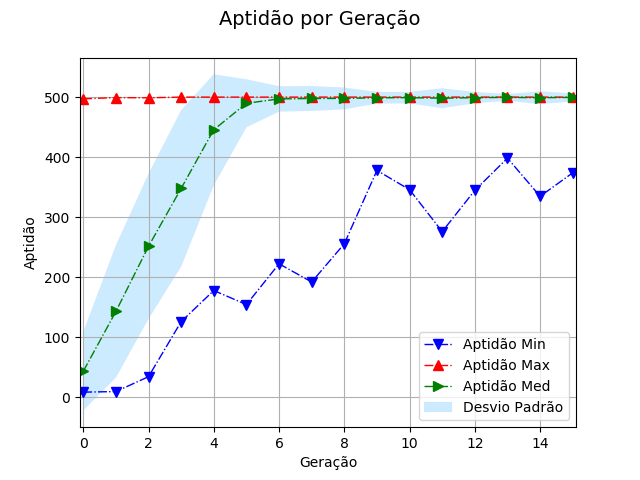
\includegraphics[width=0.8\textwidth]{02_desenvolvimento/04_EC_Fig_CartpoleAptGer.png}
	\caption{Média da aptidão de todos os indivíduos por geração (verde). Valor máximo de aptidão observado em cada geração (vermelho). Menor aptidão observada em cada geração (azul).}
	\label{fig:4ec-cartpoleaptger}
\end{figure}

Observa-se no gráfico da Figura \ref{fig:4ec-cartpoleaptger} que logo na primeira geração alguns indivíduos já são capazes de obter a aptidão máxima. Isto se deve ao grande número de indivíduos (500) gerados aleatoriamente o que funciona, de certa forma, como uma busca exaustiva totalmente aleatória.

Entretanto, é possível observar o aumento da aptidão média e mínima ao longo das gerações. O gráfico da Figura \ref{fig:4ec-cartpoleapthist} mostra o número de indivíduos que atingiram uma determinada faixa de aptidão, em cada geração.

\begin{figure}[H]
	\centering
	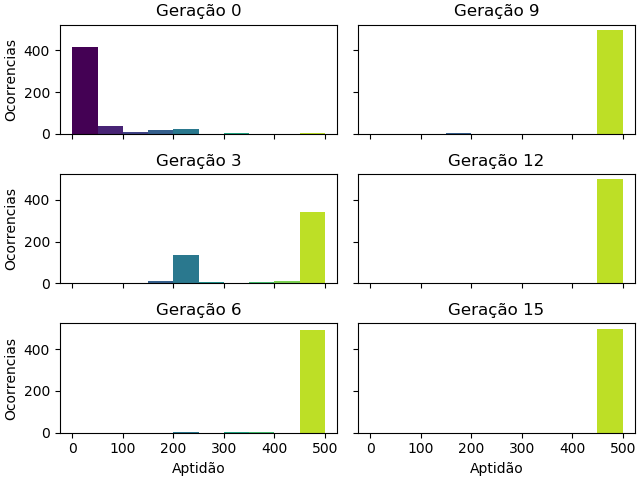
\includegraphics[width=0.8\textwidth]{02_desenvolvimento/04_EC_Fig_CartpoleAptHist.png}
	\caption{Número de indivíduos, em cada geração, que obtiveram cada faixa de aptidão. Verifica-se que já na 12º geração, a maior parte dos indivíduos possuem a aptidão máxima.}
	\label{fig:4ec-cartpoleapthist}
\end{figure}

Conforme visto no capítulo \ref{ssec:3deap-opgeneticos}, existe uma tendência de aumento do comprimento dos indivíduos ao longo do processo. O gráfico da Figura \ref{fig:4ec-cartpolecompr} mostra a média do comprimento de cada indivíduo em cada geração, assim como os valores mínimos e máximos de comprimento. Já que todas as estatísticas foram obtidas através de média de 10 execuções, o gráfico contém valores fracionários. 

\begin{figure}[H]
	\centering
	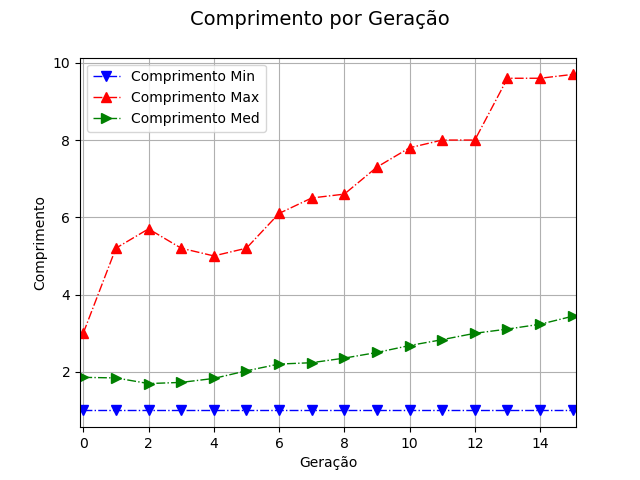
\includegraphics[width=0.8\textwidth]{02_desenvolvimento/04_EC_Fig_CartpoleCompr.png}
	\caption{Comprimento dos indivíduos por geração.}
	\label{fig:4ec-cartpolecompr}
\end{figure}

A complexidade dos indivíduos ao longo do processo pode ser observada no gráfico da Figura \ref{fig:4ec-cartpolecompl}.

\begin{figure}[H]
	\centering
	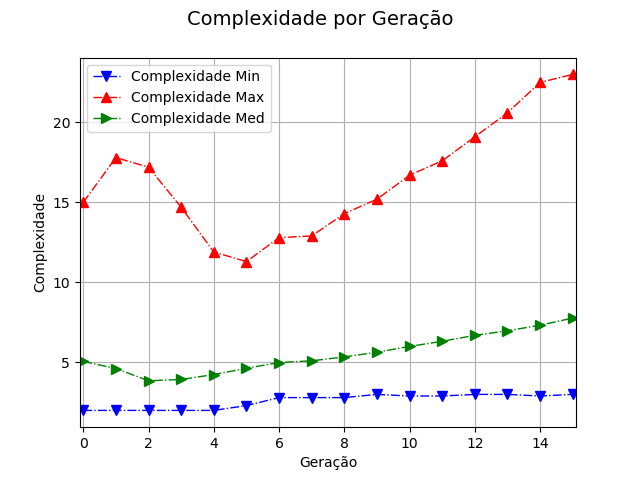
\includegraphics[width=0.8\textwidth]{02_desenvolvimento/04_EC_Fig_CartpoleCompl.png}
	\caption{As medidas relacionadas à complexidade dos indivíduos em cada geração. Essa estatística tem uma alta correlação com a aridade das operações que ocorrem nos indivíduos.}
	\label{fig:4ec-cartpolecompl}
\end{figure}

Foi possível observar que alguns operadores e variáveis, pertencentes ao conjunto primitivo, são mais eficientes para a solução do problema, e tendem a aparecer com maior frequência à medida que a população se torna mais apta. Foi realizada a contagem dos operadores e variáveis de cada indivíduo da geração final, o resultado pode ser verificado no gráfico da Figura \ref{fig:4ec-cartpoleoper}.

\begin{figure}[H]
	\centering
	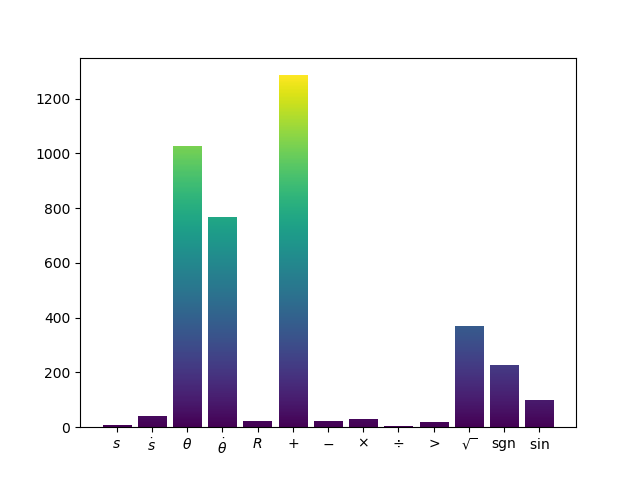
\includegraphics[width=0.8\textwidth]{02_desenvolvimento/04_EC_Fig_CartpoleOper.png}
	\caption{Ocorrência de cada operador e variável nos indivíduos da última geração.}
	\label{fig:4ec-cartpoleoper}
\end{figure}

Através do objeto \textit{hall da fama}, é possível armazenar os indivíduos mais aptos que existiram na população ao longo de todo o processo de evolução. Esse objeto é atualizado a cada geração, de modo que o primeiro indivíduo possui a maior aptidão encontrada durante toda a execução do algoritmo evolucionário. Além disso, por ser um objeto de tamanho fixo, os indivíduos de gerações mais antigas possuem prioridade.

Na Figura \ref{fig:4ec-cartpoleindiv1}, é possível ver o primeiro indivíduo do hall da fama. Já que na geração inicial alguns indivíduos obtiveram a aptidão máxima, a solução da Figura \ref{fig:4ec-cartpoleindiv1} tem prioridade sobre qualquer outra solução. O pequeno comprimento do indivíduo indica que, de fato, pertence às primeiras gerações.

\begin{figure}[H]
	\centering
	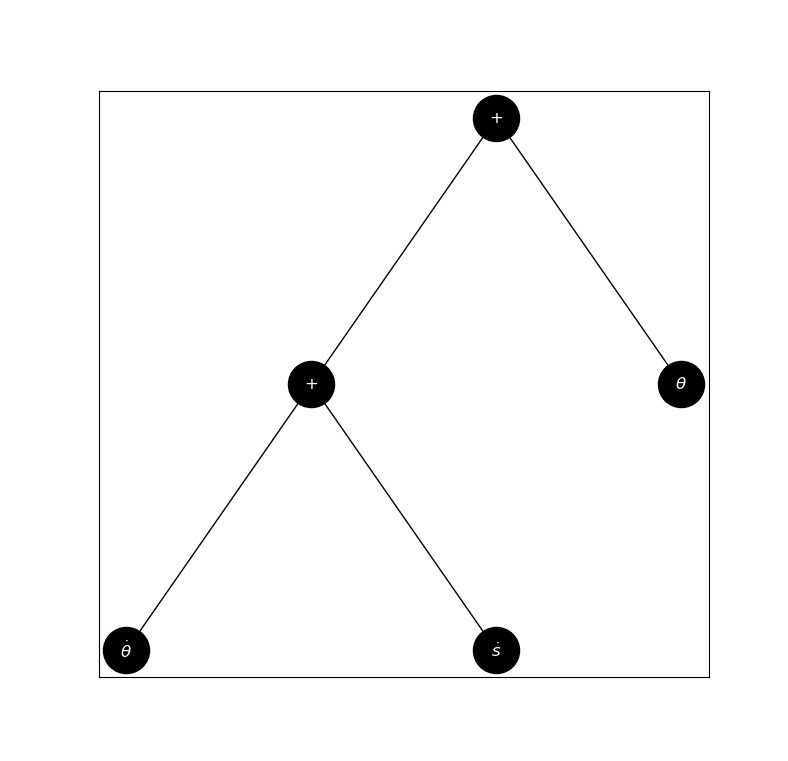
\includegraphics[width=\textwidth]{02_desenvolvimento/04_EC_Fig_CartpoleIndiv1.png}
	\caption{Primeiro indivíduo do hall da fama na primeira execução.}
	\label{fig:4ec-cartpoleindiv1}
\end{figure}

É possível perceber indivíduos de maior comprimento nas posições finais do hall da fama, como por exemplo, na Figura \ref{fig:4ec-cartpoleindiv2}.

\begin{figure}[H]
	\centering
	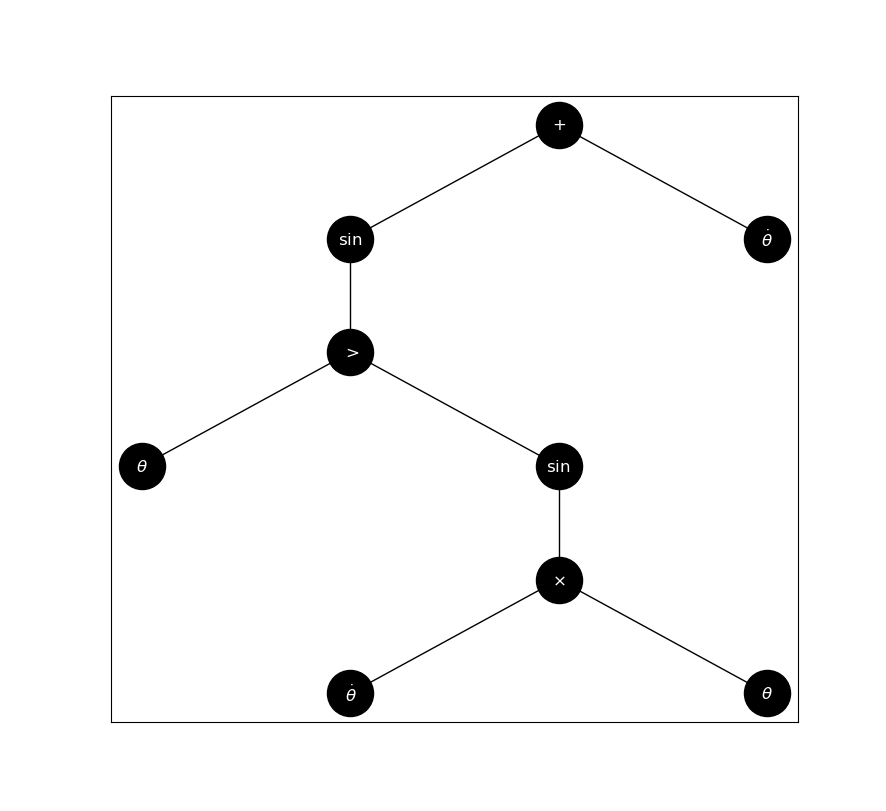
\includegraphics[width=\textwidth]{02_desenvolvimento/04_EC_Fig_CartpoleIndiv2.png}
	\caption{Vigésimo terceiro indivíduo do hall da fama, também na primeira execução do algoritmo.}
	\label{fig:4ec-cartpoleindiv2}
\end{figure}

A Figura \ref{fig:4ec-cartpolegrafaval} mostra os gráficos relacionados à avaliação do indivíduo da Figura \ref{fig:4ec-cartpoleindiv1}, em um único episódio. O eixo \textit{ação} indica o controle aplicado no ambiente a partir do \textit{resultado} de saída ao avaliar a expressão matemática da árvore.

\begin{figure}[H]
	\centering
	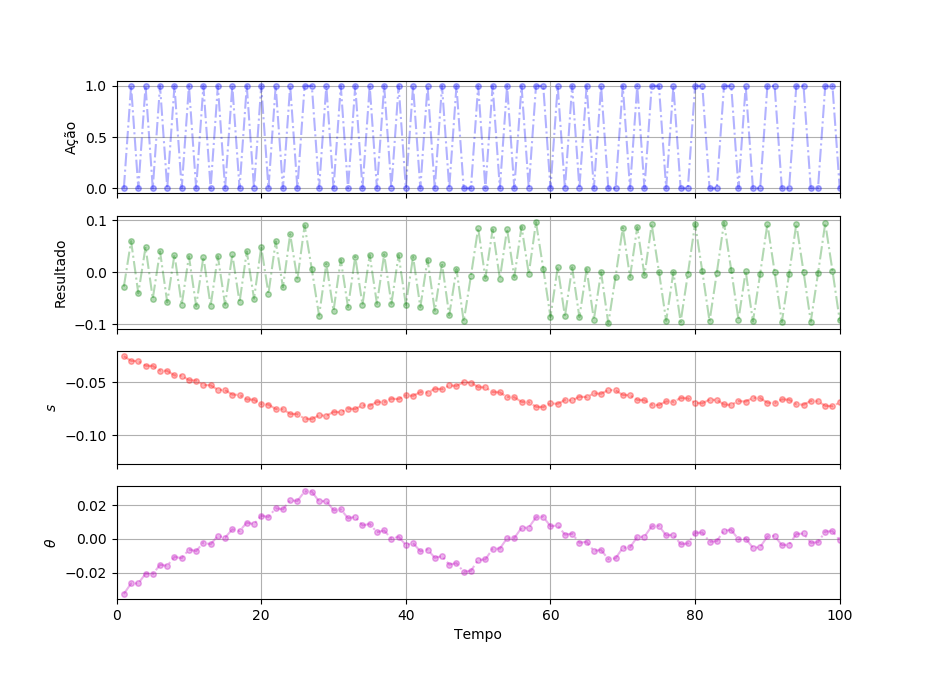
\includegraphics[width=\textwidth]{02_desenvolvimento/04_EC_Fig_CartpoleGraficosAval.png}
	\caption{Controle do pêndulo pelo indivíduo da Figura \ref{fig:4ec-cartpoleindiv1}. O pêndulo é levado rapidamente à um estado de baixa oscilação nos valores angulares.}
	\label{fig:4ec-cartpolegrafaval}
\end{figure}

Foi possível observar que os indivíduos aptos pertencentes ao hall da fama são capazes de manter um valor baixo de oscilação do ângulo ao redor do zero, entretanto, algumas soluções causavam a posição do carrinho a tender para um dos extremos, o que pode levar ao término antecipado do episódio. 

Já que as aptidões dos indivíduos foram estimadas a partir de 10 simulações, é possível que as melhores soluções tenham sido beneficiadas por condições iniciais vantajosas. Não é possível, entretanto, aumentar o número de simulações sem que haja aumento considerável no tempo de execução do algoritmo.

Dessa forma, é interessante verificar a aptidão dos indivíduos do hall da fama, em um grande número de episódios. Dessa forma, encontraremos o indivíduo mais apto para qualquer condição inicial.

É proveitoso realizar, nesse momento, a comparação desses resultados com a abordagem proposta pelo algoritmo DQN, uma vez que a medida de aptidão é a mesma. O tempo médio de execução do algoritmo de PG foi \SI{334}{s}. O agente DQN será treinado, aproximadamente, pelo mesmo tempo. Em seguida, as recompensas médias acumuladas por episódio, em 100 simulações serão comparadas. Destaca-se que a avaliação da PG foi realizada pela média de recompensa acumulada pelos 10 primeiros membros do hall da fama.

Utilizando a biblioteca \textit{stable-baselines} \cite{stable-baselines}, o agente foi treinado por \SI{334}{s} (código no apêndice). O gráfico da Figura \ref{fig:4ec-cartpoledqndiverg} mostra a recompensa obtida pelo agente ao longo do treinamento.

\begin{figure}[H]
	\centering
	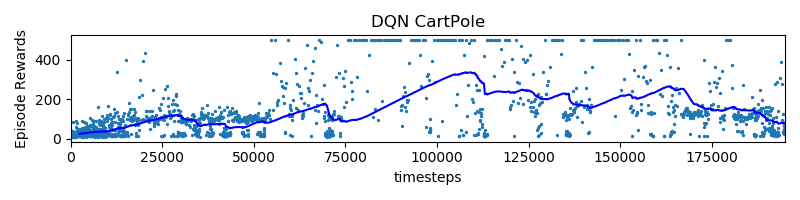
\includegraphics[width=0.85\textwidth]{02_desenvolvimento/04_EC_Fig_CartpoleDQNDiverg.png}
	\caption{Recompensa média acumulada em função do número de passos de simulação. A linha azul representa a média móvel.}
	\label{fig:4ec-cartpoledqndiverg}
\end{figure}

Na Figura \ref{fig:4ec-cartpoledqndiverg} é possível notar a degradação da recompensa média acumulada a partir dos 110000 passos de simulação. Já que a rede neural tende a exibir esse comportamento, sem a devida otimização dos hiperparâmetros, o algoritmo foi executado novamente com o número de passos totais reduzido. O resultado pode ser verificado na Figura \ref{fig:4ec-cartpoledqngraf}.

\begin{figure}[H]
	\centering
	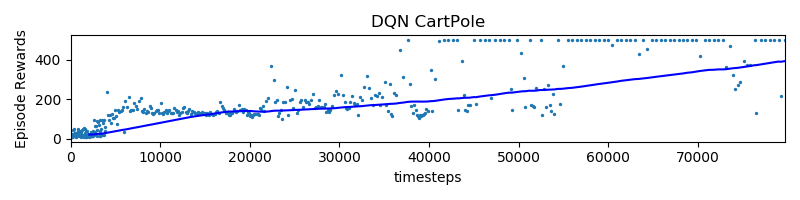
\includegraphics[width=0.85\textwidth]{02_desenvolvimento/04_EC_Fig_CartpoleDQNGraf.png}
	\caption{Recompensa média ao longo dos passos de simulação e a média móvel.}
	\label{fig:4ec-cartpoledqngraf}
\end{figure}

A Tabela \ref{tab:4ec-cartpolecomp} sumariza uma breve comparação entre o desempenho da programação genética com o algoritmo DQN, em termos de custos computacionais.

\begin{table}[H]
	\centering
	\begin{tabular}{SSS} \toprule
		{} & {\textbf{PG}} & {\textbf{DQN}} \\ \midrule
		{\textbf{Desempenho}} & {497} & {500} \\
		{\textbf{Tempo de execução (s)}} & {334} & {280} \\
		{\textbf{Passos de simulação}} & {16647338} & {80000} \\
		{\textbf{Número de episódios}} & {65095} & {450\footnotemark} \\
		\bottomrule
	\end{tabular}
	\caption{Comparação entre a programação genética e DQN para o pêndulo invertido.}\label{tab:4ec-cartpolecomp}
\end{table}

\footnotetext[1]{Valor estimado.}

A Figura \ref{fig:4ec-cartpoledqnvargraf} mostra a atuação do agente DQN ao longo de um episódio.

\begin{figure}[H]
	\centering
	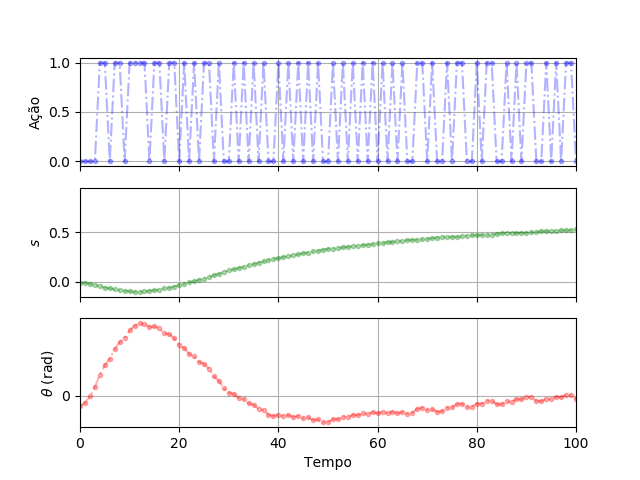
\includegraphics[width=0.85\textwidth]{02_desenvolvimento/04_EC_Fig_CartpoleDQNVarGraf.png}
	\caption{Posição do carrinho (topo) e ângulo do bastão em função do tempo.}
	\label{fig:4ec-cartpoledqnvargraf}
\end{figure}

Observamos, por fim, que as duas abordagens foram capazes de encontrar soluções satisfatórias para o problema. A seguir, serão abordados outros problemas que envolvem pêndulos e sua estabilização. 

\subsection{Pêndulo \textit{Swing-up}}\label{ssec:4ec-pendulum}

O próximo sistema simulado esta disponível na biblioteca Gym, na seção \textit{classic control}, direcionada à implementação de ambientes de simulações para problemas clássicos de controle. Conforme a abordagem do problema anterior, serão introduzidos os critérios de término do episódio, as variáveis de estado observáveis e a implementação da recompensa. A formulação da função de aptidão, a partir da recompensa disponível também será abordada.

A dinâmica envolve um bastão com uma de suas extremidades fixadas, sendo possível a atuação do agente a partir da aplicação de um torque, em qualquer sentido, buscando a manutenção da extremidade livre na posição mais alta, ou seja, o pêndulo deve ser mantido verticalmente para cima. A Figura \ref{fig:4ec-pendulumenv} ilustra o problema.

\begin{figure}[H]
	\centering
	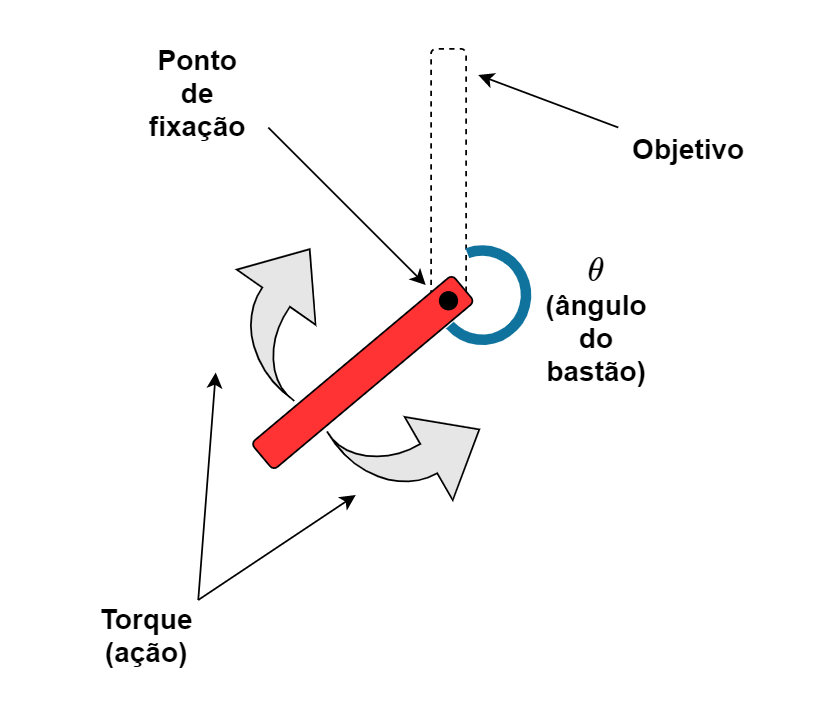
\includegraphics[width=0.7\textwidth]{02_desenvolvimento/04_EC_Fig_PendulumEnv2.png}
	\caption{Pêndulo \textit{Swing-up}.}
	\label{fig:4ec-pendulumenv}
\end{figure}

A seguir serão enumerados alguns aspectos que tornam o problema mais complexo e outras diferenças fundamentais do ambiente, em comparação com o pêndulo invertido:

\begin{itemize}[label=\raisebox{0.25ex}{\tiny$\bullet$}]
	\item O ponto de equilíbrio é estável.
	\item O torque aplicado em um único sentido, a partir da posição de repouso, não é capaz de alcançar o objetivo em um movimento contínuo (o bastão precisa adquirir momento para superar a força gravitacional).
	\item As ações possíveis se dão no espaço contínuo.
	\item As recompensas são implementadas a partir de uma função custo.
\end{itemize}

A Tabela \ref{tab:4ec-pendulumvarestado} sumariza as variáveis de estado do sistema, que são fornecidas como uma \textit{observação} após cada ação do agente. Já que o ponto de equilíbrio do sistema é estável, o único critério de término é o tempo de simulação. Com base na documentação da biblioteca Gym \cite{openaigym}, o episódio termina após 200 passos de tempo. 

\begin{table}[!htb]
	\centering
	\caption{Variáveis de estado para o pêndulo swing-up.}
	\label{tab:4ec-pendulumvarestado}
	\begin{tabular}{SS} \toprule
		{Variável} & {Significado}\\ \midrule
		{$\cos(\theta)$} & {Cosseno do ângulo do bastão} \\
		{$\sin(\theta)$} & {Seno do ângulo do bastão} \\
		{$\dot{\theta}$} & {Velocidade angular do bastão} \\ 
		\bottomrule
	\end{tabular}
\end{table}

Seguindo a abordagem da seção \ref{ssec:3deap-avalind}, será criada uma função de aptidão para o indivíduo. A recompensa a cada instante de tempo é uma função custo, que penaliza desvios do objetivo.

\begin{align}\label{eq:4ec-pendulumrewardfunction}
	\begin{split}
		r(t) = - \left[(\theta(t))^2 + 0.1(\dot\theta(t))^2+0.001(a(t))^2\right]\qquad &-\pi \le \theta \le \pi\\\\
															 	  &-2 \le a(t) \le 2
	\end{split}
\end{align}

A variável $a(t)$ representa a ação (torque) do agente no instante de tempo $t$. Foi mencionado na seção \ref{sec:1pg-apg} a possibilidade de projetar a aptidão de um indivíduo a partir de uma função custo, dessa forma, a aptidão será dada pela soma dos custos (implementados como recompensas negativas) ao longo de um episódio:

\begin{align}\label{eq:4ec-pendulumaptidao}
	\begin{split}
		A(t) &= r(t) = - \left[(\theta(t))^2 + 0.1(\dot\theta(t))^2+0.001(a(t))^2\right]\\\\
		A_{tot}^{ep} &= \sum_{t=0}^{T} A(t) = - \sum_{t=0}^{T} \left[
		(\theta(t))^2 + 0.1(\dot\theta(t))^2+0.001(a(t))^2
		\right]\qquad T \le 200\\\\
		\bar{A} &= \dfrac{1}{nep}\sum_{ep=1}^{nep} A_{tot}^{ep} = 
		-\dfrac{1}{nep}\sum_{ep=1}^{nep}\sum_{t=0}^{T} \left[
		(\theta(t))^2 + 0.1(\dot\theta(t))^2+0.001(a(t))^2
		\right]
	\end{split}
\end{align}

De forma semelhante ao problema do pêndulo invertido, o objetivo será \underline{maximizar} a aptidão média na Equação \ref{eq:4ec-pendulumaptidao}. 

Buscando demonstrar a robustez do método, poucas mudanças foram realizadas nos hiperparâmetros da Tabela \ref{tab:4ec-param-cartpole}, mais especificamente, foram alterados: o número de entradas, comprimentos de inicialização e o comprimento máximo de mutação. 

\begin{table}[H]
	\centering
	\begin{tabular}{SSS} \toprule
		{Parâmetro} & {Valor} \\ \midrule
		{Tamanho da População} & {500} \\
		{Probabilidade de Cruzamento} & {0.75} \\
		{Probabilidade de Mutação} & {0.05} \\
		{Número de Gerações} & {15} \\
		{Número de Entradas} & {3} \\
		{Faixa para Constante Efêmera} & {(-1.0, 1.0)} \\
		{Número de Simulações} & {10} \\
		{Tamanho do Campeonato de Aptidão} & {6} \\
		{Tamanho do Campeonato de Comprimento} & {1.2} \\
		{Operações} & {add, sub, mul, div, sr, cr, cos, gt, sgn} \\
		{Comprimento Mínimo e Máximo de Inicialização} & {(2, 5)} \\
		{Comprimento Máximo de Mutação} & {7} \\
		{Limite de Comprimento dos Indivíduos} & {17} \\
		\bottomrule
	\end{tabular}
	\caption{Parâmetros da programação genética aplicada ao pêndulo swing-up.}\label{tab:4ec-pendulumparam}
\end{table}

É interessante destacar que o problema da seção \ref{ssec:4ec-cartpole} utilizava ações discretas. Um mapeamento simples de números resultantes da avaliação da árvore para ações foi utilizado: números positivos produziam uma força para a direita no carrinho, enquanto que números negativos geravam uma força de sentido contrário. 

Neste problema, o espaço de ações é contínuo, portanto é necessário apenas garantir que o resultado matemático da compilação de um indivíduo obedeça os limites de torque definidos na equação \ref{eq:4ec-pendulumrewardfunction}. Isto pode ser concebido pela utilização da função \textit{clip}, cujo comportamento é demonstrado na Figura \ref{fig:4ec-pendulumclip}.

\begin{figure}[H]
	\centering
	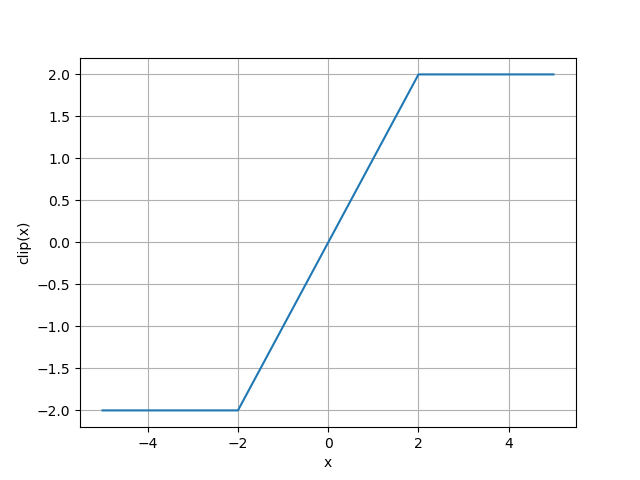
\includegraphics[width=0.82\textwidth]{02_desenvolvimento/04_EC_Fig_PendulumClipFun.png}
	\caption{Função \textit{clip}.}
	\label{fig:4ec-pendulumclip}
\end{figure}

Essa função funcionará como \textit{wrapper}, isto é, um mapeamento do resultado de avaliação da árvore para uma ação dentro do espaço de ações possíveis.

Novamente, o algoritmo foi executado 10 vezes e a média das estatísticas relevantes foram obtidas. A começar pela aptidão ao longo das gerações, onde é possível perceber que a busca inicial da primeira geração, através da inicialização, não é capaz de obter um resultado satisfatório como no problema anterior. Porém, as próximas gerações encontram uma solução eficaz para o pêndulo, conforme pode ser visto nas Figuras \ref{fig:4ec-pendulumaptger} e \ref{fig:4ec-pendulumapthist}.

\begin{figure}[H]
	\centering
	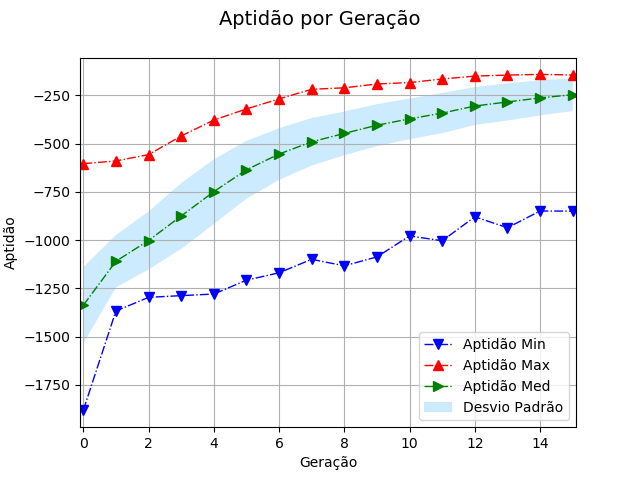
\includegraphics[width=0.85\textwidth]{02_desenvolvimento/04_EC_Fig_PendulumAptGer.png}
	\caption{Aptidão dos indivíduos ao longo das gerações.}
	\label{fig:4ec-pendulumaptger}
\end{figure}

\begin{figure}[H]
	\centering
	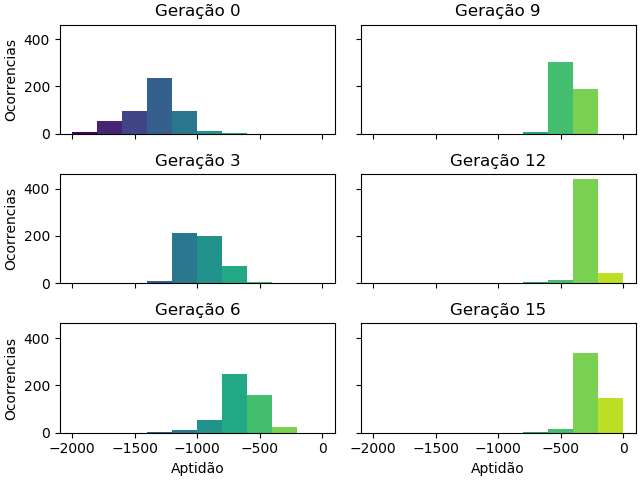
\includegraphics[width=0.85\textwidth]{02_desenvolvimento/04_EC_Fig_PendulumAptHist.png}
	\caption{Histograma da aptidão dos indivíduos em cada geração.}
	\label{fig:4ec-pendulumapthist}
\end{figure}

O comprimento e a complexidade dos indivíduos da população, ao longo das gerações, podem ser vistos nas Figuras \ref{fig:4ec-pendulumcompr} e \ref{fig:4ec-pendulumcompl}, respectivamente.

\begin{figure}[H]
	\centering
	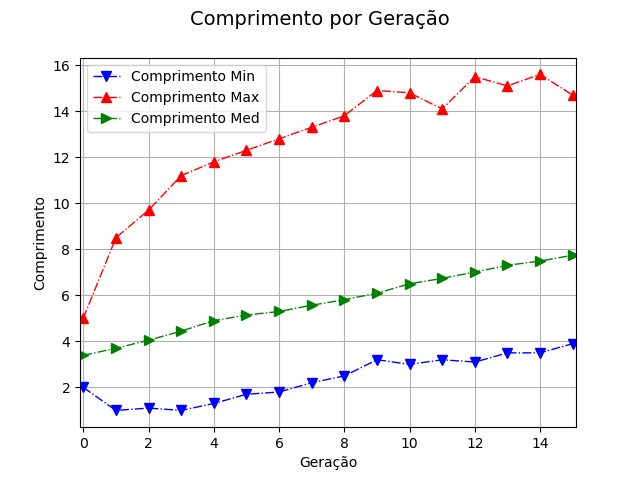
\includegraphics[width=0.85\textwidth]{02_desenvolvimento/04_EC_Fig_PendulumCompr.png}
	\caption{Comprimento dos indivíduos ao longo das gerações.}
	\label{fig:4ec-pendulumcompr}
\end{figure}

\begin{figure}[H]
	\centering
	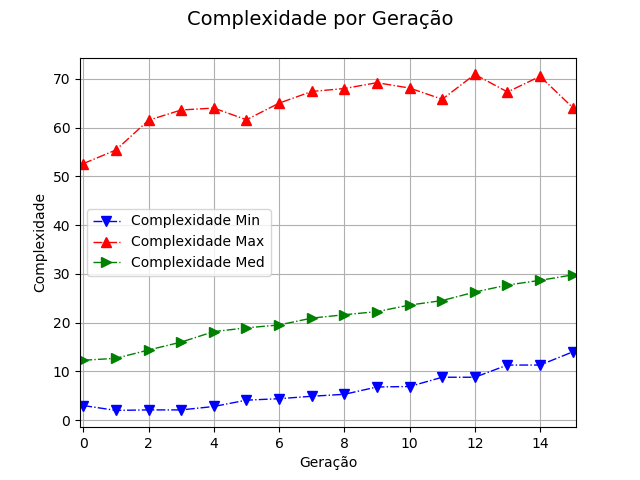
\includegraphics[width=0.85\textwidth]{02_desenvolvimento/04_EC_Fig_PendulumCompl.png}
	\caption{Medida da complexidade dos indivíduos em cada geração.}
	\label{fig:4ec-pendulumcompl}
\end{figure}

É possível perceber o aumento dessas duas medidas em relação ao pêndulo invertido, devido também à mudanças na inicialização e no comprimento máximo da mutação. 

A Figura \ref{fig:4ec-pendulumoper} mostra o histograma de ocorrência dos operadores e variáveis terminais na população da última geração. 

\begin{figure}[H]
	\centering
	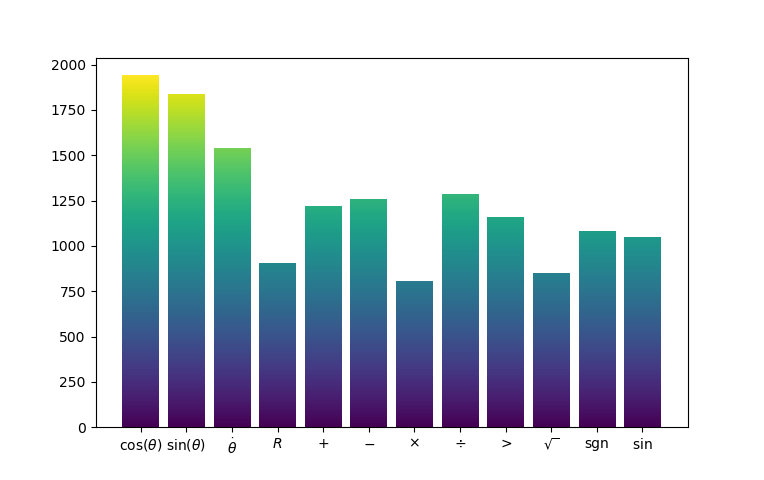
\includegraphics[width=0.85\textwidth]{02_desenvolvimento/04_EC_Fig_PendulumOper.png}
	\caption{Histograma de operadores e variáveis terminais na última geração.}
	\label{fig:4ec-pendulumoper}
\end{figure}

O indivíduo de maior aptidão observado, na primeira execução, é mostrado na Figura \ref{fig:4ec-pendulumindiv1}.

\begin{figure}[H]
	\centering
	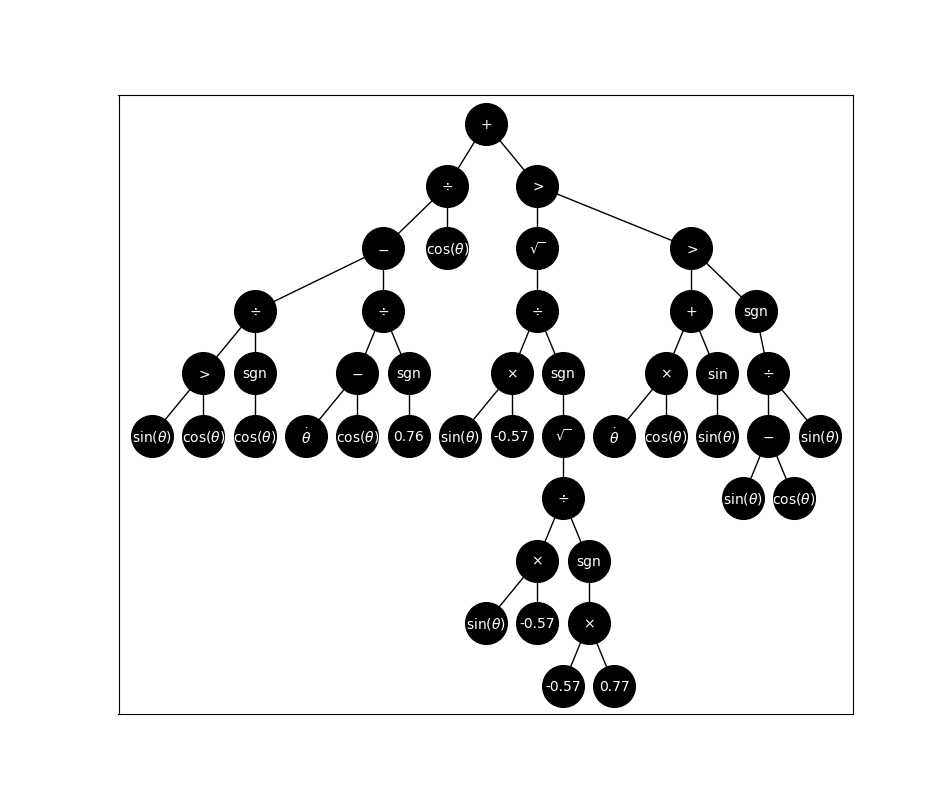
\includegraphics[width=\textwidth]{02_desenvolvimento/04_EC_Fig_PendulumIndiv1.png}
	\caption{Primeiro integrante do hall da fama.}
	\label{fig:4ec-pendulumindiv1}
\end{figure}

O segundo integrante do hall da fama, na primeira execução, é mostrado na Figura \ref{fig:4ec-pendulumindiv2}.

\begin{figure}[H]
	\centering
	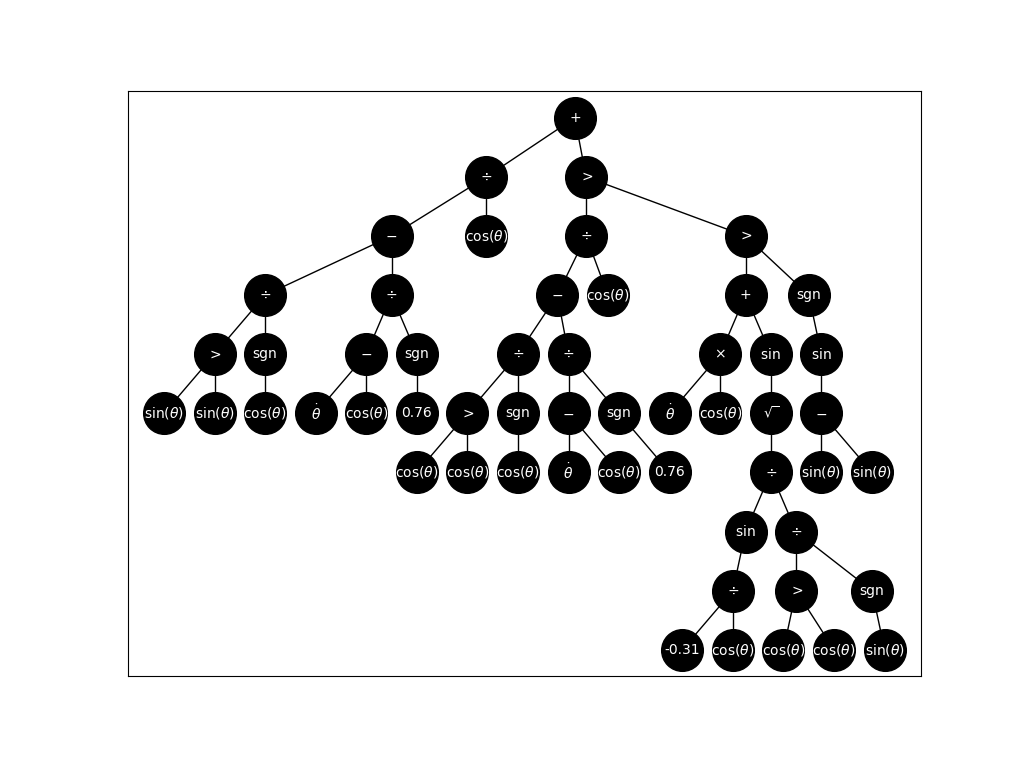
\includegraphics[width=\textwidth]{02_desenvolvimento/04_EC_Fig_PendulumIndiv2.png}
	\caption{Segundo integrante do hall da fama.}
	\label{fig:4ec-pendulumindiv2}
\end{figure}

A Figura \ref{fig:4ec-pendulumgraficosaval} mostra as variáveis relevantes ao avaliar o indivíduo da Figura \ref{fig:4ec-pendulumindiv1} em um episódio. 

\begin{figure}[H]
	\centering
	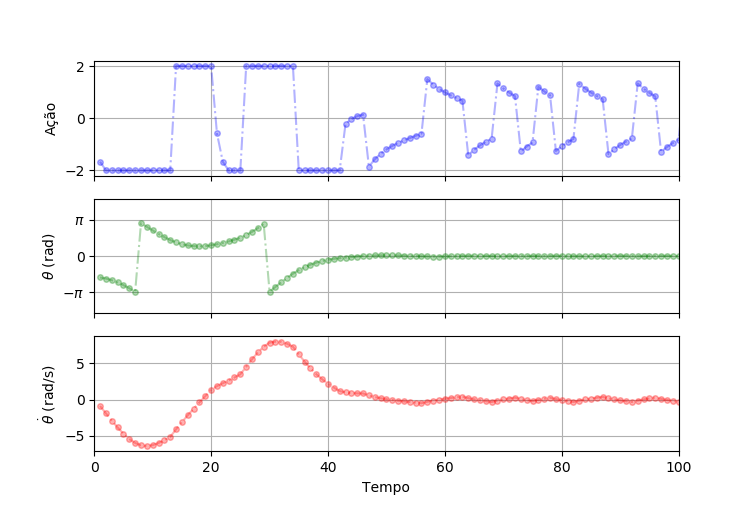
\includegraphics[width=0.95\textwidth]{02_desenvolvimento/04_EC_Fig_PendulumGraficosAval.png}
	\caption{Controle exercido pelo indivíduo da Figura \ref{fig:4ec-pendulumindiv1}.}
	\label{fig:4ec-pendulumgraficosaval}
\end{figure}

As transições bruscas no ângulo $\theta$ indicam a passagem da extremidade livre do pêndulo no ponto mais baixo, onde o custo adquiri seu valor máximo. Após esse momento, o ângulo oscila em torno do zero de forma estável.

Utilizando a mesma metodologia da seção \ref{ssec:4ec-cartpole}, será feita uma avaliação em 100 episódios dos indivíduos do hall da fama. O maior valor de aptidão obtido será comparado com a recompensa acumulada de um agente treinado com o algoritmo DDPG, que pode ser visto como uma extensão do algoritmo DQN para ambientes com ações no espaço contínuo. Novamente, a medida de desempenho de um agente ou indivíduo é a função de recompensa disponibilizada pelo ambiente de simulação. Com isso, é possível realizar uma comparação direta entre as duas abordagens.

A Figura \ref{fig:4ec-pendulumddpggraf} mostra o agente DDPG sendo treinado em 100000 passos de tempo.

\begin{figure}[H]
	\centering
	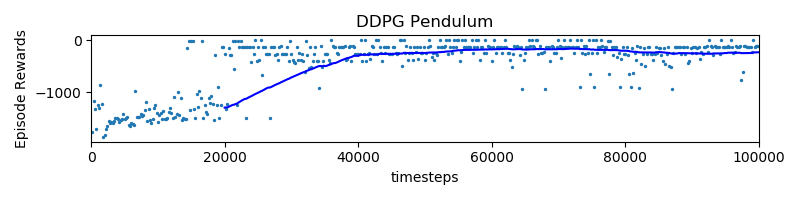
\includegraphics[width=0.9\textwidth]{02_desenvolvimento/04_EC_Fig_PendulumDDPGGraf.png}
	\caption{Evolução da recompensa acumulada para o agente DDPG no pêndulo swing-up.}
	\label{fig:4ec-pendulumddpggraf}
\end{figure}

A atuação do agente em um episódio pode ser vista na Figura \ref{fig:4ec-pendulumddpgvargraf}. 

\begin{figure}[H]
	\centering
	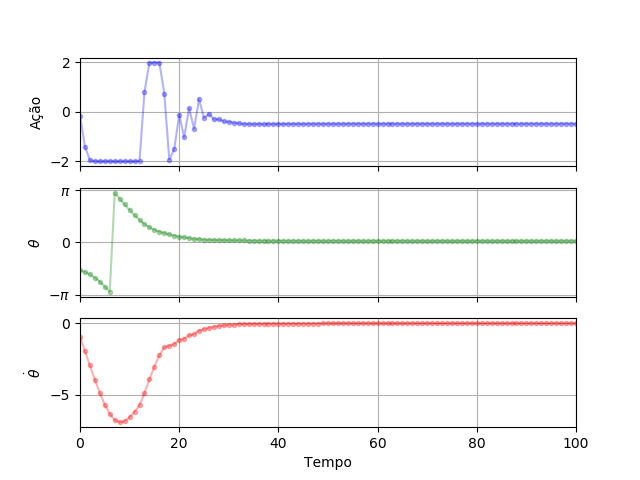
\includegraphics[width=0.9\textwidth]{02_desenvolvimento/04_EC_Fig_PendulumDDPGVarGraf.png}
	\caption{Dinâmica do pêndulo swing-up sob ação do agente DDPG.}
	\label{fig:4ec-pendulumddpgvargraf}
\end{figure}

\begin{table}[H]
	\centering
	\begin{tabular}{SSS} \toprule
		{} & {\textbf{PG}} & {\textbf{DDPG}} \\ \midrule
		{\textbf{Desempenho}} & {-230} & {-253} \\
		{\textbf{Tempo de execução (s)}} & {1649} & {194} \\
		{\textbf{Passos de simulação}} & {13034400} & {100000} \\
		{\textbf{Número de episódios}} & {65172} & {500} \\
		\bottomrule
	\end{tabular}
	\caption{Comparação entre a programação genética e DDPG para o pêndulo swing-up.}\label{tab:4ec-pendulumcomp}
\end{table}

É possível notar a partir da Tabela \ref{tab:4ec-pendulumcomp} que as duas abordagens são capazes de resolver o problema de controle proposto.

\subsection{Pêndulo Duplo Invertido}\label{ssec:4ec-dp}

Este problema é similar ao pêndulo invertido, pois a estabilização do bastão envolve a movimentação do objeto (que contém o ponto de fixação) em uma trilha. A diferença reside na existência de um outro bastão, fixado na extremidade antes livre, aumentando consideravelmente a complexidade do problema. A Figura \ref{} mostra o sistema proposto, em um ambiente tridimensional.

\begin{figure}[H]
	\centering
	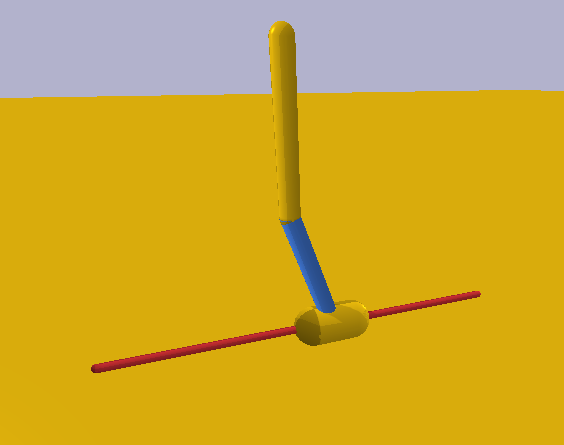
\includegraphics[width=0.8\textwidth]{02_desenvolvimento/04_EC_Fig_DPEnv.png}
	\caption{Renderização 3D do sistema pêndulo duplo invertido.}
	\label{fig:4ec-dpenv}
\end{figure}

A observação do sistema é composta por 11 variáveis:

\begin{table}[H]
	\centering
	\caption{Variáveis de estado para o pêndulo duplo invertido.}
	\label{tab:4ec-dpvarestado}
	\begin{tabular}{SS} \toprule
		{Variável} & {Significado}\\ \midrule
		{$s$} & {Posição do carrinho} \\
		{$\sin(\theta)$} & {Seno do ângulo do bastão inferior} \\
		{$\sin{(\gamma)}$} & {Seno do ângulo do bastão superior} \\ 
		{$\cos(\theta)$} & {Cosseno do ângulo do bastão inferior} \\
		{$\cos(\gamma)$} & {Cosseno do ângulo do bastão superior} \\
		{$\dot{s}$} & {Velocidade do carrinho} \\
		{$\dot{\theta}$} & {Velocidade angular do bastão inferior} \\
		{$\dot{\gamma}$} & {Velocidade angular do bastão superior} \\
		{$f_r(s)$} & {Força de restrição em função da posição} \\
		{$f_r(\theta)$} & {Força de restrição em função de $\theta$} \\
		{$f_r(\gamma)$} & {Força de restrição em função de $\gamma$} \\
		\bottomrule
	\end{tabular}
\end{table}

Conforme a abordagem realizada até o momento, todas as variáveis da Tabela \ref{tab:4ec-dpvarestado} farão parte do conjunto primitivo. Os outros parâmetros foram mantidos iguais ao do problema anterior (Tabela \ref{tab:4ec-pendulumparam}).

A função de recompensa do ambiente de simulação, a cada instante de tempo, é dada na equação (\ref{eq:4ec-dprewardfunction}).

\begin{align}\label{eq:4ec-dprewardfunction}
	\begin{split}
		r(t) &= 10 - d_p(t) - v_p(t)\\\\
		d_p(t) &= 0.01(s(t))^2 + (y(t)-2)^2\\\\
		v_p(t) &= 0.001(\dot{\theta}(t))^2 + 0.005(\dot{\gamma}(t))^2
	\end{split}
\end{align}

Na equação (\ref{eq:4ec-dprewardfunction}), $d_p(t)$ e $v_p(t)$ são penalidades dadas em função da distância e das velocidades angulares dos bastões, respectivamente. A variável $y$ representa a altura da extremidade livre do bastão superior. Além de auxiliar o cálculo do custo, a quantidade $y$ também auxilia na verificação do término do episódio. Mais especificamente, a simulação encerra após 1000 passos de tempo ou quando a variável $y$ assume valores menores ou iguais a 1.

Naturalmente, a recompensa da equação (\ref{eq:4ec-dprewardfunction}) será utilizada para o cálculo da aptidão de um indivíduo. Utilizando a mesma formulação das equações em (\ref{eq:4ec-pendulumaptidao}):

\begin{align}\label{eq:4ec-dpaptidao}
	\begin{split}
		A(t) &= r(t) = 10 - d_p(t) - v_p(t)\\\\
		A_{tot}^{ep} &= \sum_{t=0}^{T} A(t) = - \sum_{t=0}^{T} \left[
		10 - d_p(t) - v_p(t)
		\right]\qquad T \le 1000\\\\
		\bar{A} &= \dfrac{1}{nep}\sum_{ep=1}^{nep} A_{tot}^{ep} = 
		-\dfrac{1}{nep}\sum_{ep=1}^{nep}\sum_{t=0}^{T} 
		\left[
		10 - d_p(t) - v_p(t)
		\right]
	\end{split}
\end{align}

Como o espaço de ações é contínuo, será utilizada a função clip, da Figura \ref{fig:4ec-pendulumclip}, como wrapper para o resultado compilado dos indivíduos. Entretanto, os valores extremos serão $-1$ e $1$. 

As Figuras \ref{fig:4ec-dpapthist} a \ref{fig:4ec-dpcompl} mostram os resultados obtidos, através de 10 execuções do algoritmo.

\begin{figure}[H]
	\centering
	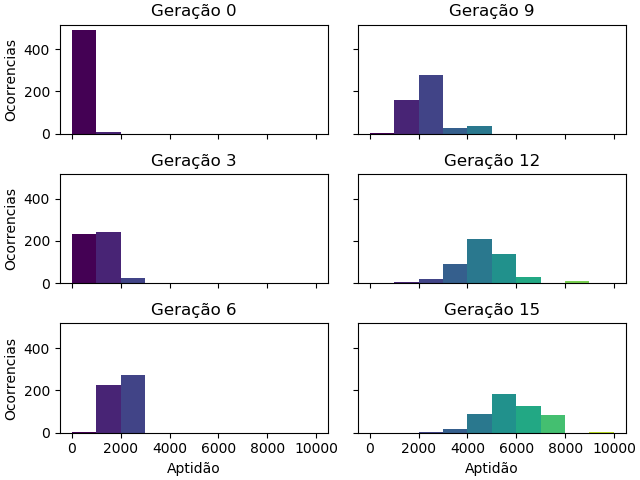
\includegraphics[width=0.8\textwidth]{02_desenvolvimento/04_EC_Fig_DPAptHist.png}
	\caption{Histograma da aptidão dos indivíduos, em algumas gerações, para o pêndulo duplo invertido.}
	\label{fig:4ec-dpapthist}
\end{figure}

\begin{figure}[H]
	\centering
	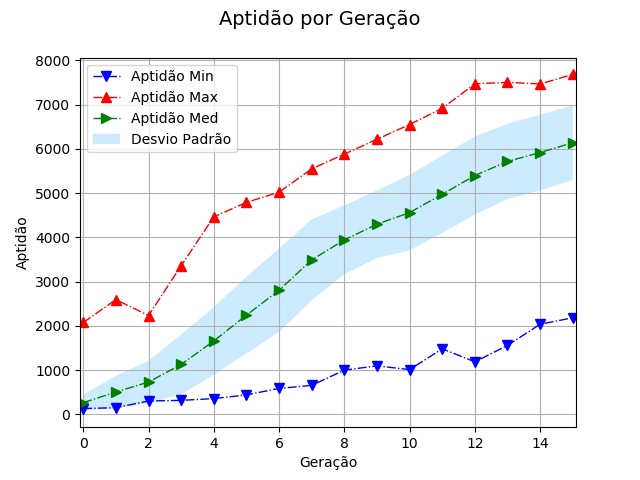
\includegraphics[width=0.8\textwidth]{02_desenvolvimento/04_EC_Fig_DPAptGer.png}
	\caption{Medidas de aptidão da população, em cada geração.}
	\label{fig:4ec-dpaptger}
\end{figure}

\begin{figure}[H]
	\centering
	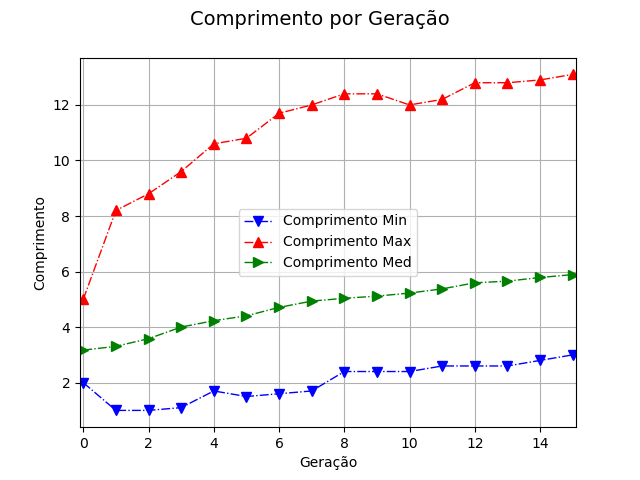
\includegraphics[width=0.8\textwidth]{02_desenvolvimento/04_EC_Fig_DPCompr.png}
	\caption{Medidas de comprimento da população ao longo das gerações.}
	\label{fig:4ec-dpcompr}
\end{figure}

\begin{figure}[H]
	\centering
	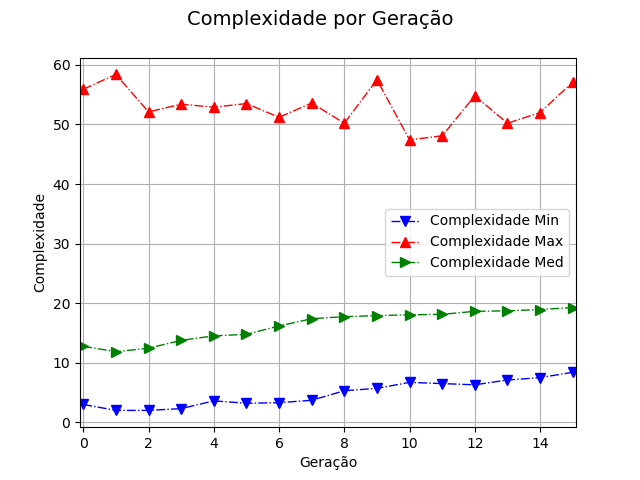
\includegraphics[width=0.8\textwidth]{02_desenvolvimento/04_EC_Fig_DPCompl.png}
	\caption{Medidas de complexidade dos indivíduos em função das gerações.}
	\label{fig:4ec-dpcompl}
\end{figure}

Para cada indivíduo do hall da fama, conforme feito anteriormente, 100 simulações foram realizadas, com o intuito de verificar a solução mais apta e generalista. O indivíduo da Figura \ref{fig:4ec-dpindiv1} obteve uma aptidão média de 7794.

\begin{figure}[H]
	\centering
	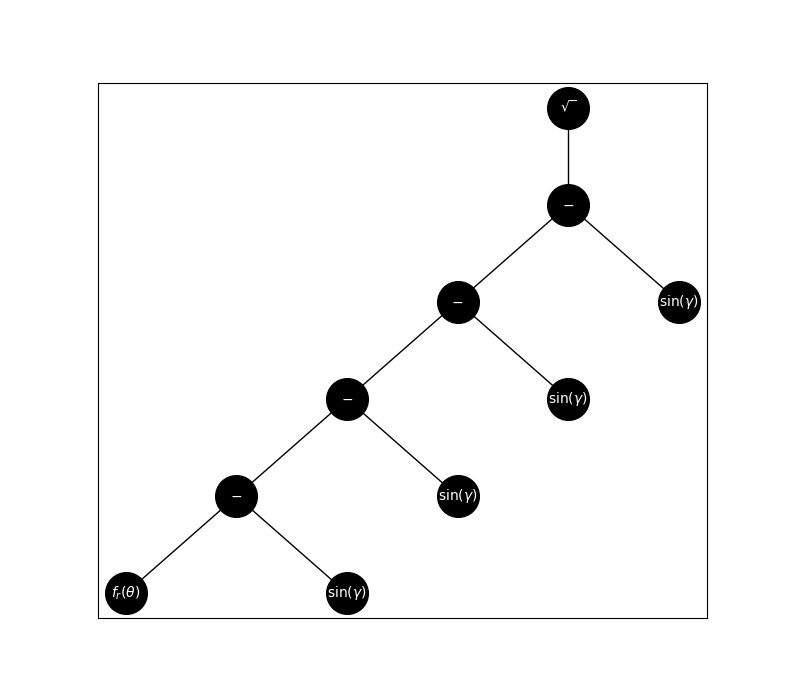
\includegraphics[width=0.9\textwidth]{02_desenvolvimento/04_EC_Fig_DPIndiv1}
	\caption{Indivíduo mais apto da primeira execução do algoritmo.}
	\label{fig:4ec-dpindiv1}
\end{figure}

Os gráficos da Figura \ref{fig:4ec-dpvargraf} mostra os ângulos e a posição do carrinho, quando a solução da Figura \ref{fig:4ec-dpindiv1} atua. 

\begin{figure}[H]
	\centering
	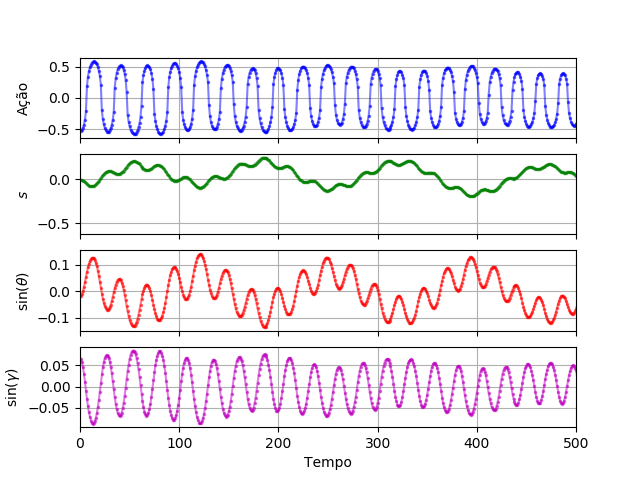
\includegraphics[width=0.9\textwidth]{02_desenvolvimento/04_EC_Fig_DPVarGraf}
	\caption{Avaliação do melhor indivíduo observado na primeira execução.}
	\label{fig:4ec-dpvargraf}
\end{figure}























